%!TEX root = paper.tex
%%%%%%%%%%%%%%%%%%%%%%%%%%%%%%%%%%%%%%%%%%%%%%%%%%%%%%%%%%%%%%%%%%%%%%%%%%%%%%%%
\section{Simulation and Scenario Evaluation}
\label{sec:simulation}

Based on the models introduced in Section~\ref{sec:model} a stochastic 
\gls{DES} was created. This 
\textsc{Gnu R}-based simulator strives to translate all of the earlier 
discussed components of lag, while keeping them as configurable as possible.
%By using a vector-based language the core loop is kept compact and easy to modify in order to adapt to new scenarios in addition to the ones evaluated here. 
Due to the influence of several stochastic processes (user inputs $U$, network delay $D$, server processing time $P$) and the differing offset of the clocked processes, a sufficient number of repetitions is required to provide meaningful results. This is achieved by running large numbers of simulations 
in parallel through the built-in R facilities.

This section presents simulation results on each of the flavors of how to play video games: the local, online, and the cloud scenario.
The investigations here are not intended to cover every aspect of all parameters or to conduct full parameter studies, but are rather to highlight some particular aspect in each of the scenario. 

All of the source code and the data from the upcoming scenarios is provided in the simulation folder\footnote{\url{https://github.com/mas-ude/onlinegame-lag-sim/tree/master/simulation}} of the repository and can be used as public domain.


\subsection{Parameters}

Besides being fully reconfigurable, the simulation currently also has a few default parameters set and makes assumptions that go beyond what the base end-to-end model implies for reasons of simplicity. They are chosen to be as realistic as possible and and are summarized in Table~\ref{tab:notation}.
%\hoss{Vielleicht noch kurz erwaehnen, dass die Parameter realistisch gewaehlt sind? Gibt es dafuer Referenzen?}
% fm: referenzen für solche werte sind leider eher schwer zu finden

First, the input is modeled by an exponential distribution with a rate of $20$ events per second. The offsets between the clocked processes are uniformly distributed in their respective intervals. It is further assumed that the server processing time $P$ follows a left-truncated normal distribution with $\mu_P = \SI{3}{\milli\second}$ and $\sigma_P = \SI{0.1}{\milli\second}$.
%\textbf{TODO:} implications and reasons?
Additionally, the rate $c$ at which command messages are sent to the game server is set equal to the server's tickrate $g$ as the server would not process more commands either way. This might however increase the end-to-end lag in some situations if a command message just misses one of the server's ticks and has to wait another full cycle.

The evaluation of the presented scenarios was conducted on the basis of $r=\np{1000}$ repetitions for each setting. Each run $i \in \{1,\dots,r\}$ consisted of a series of $n=\np{100}$ input events and their associated end-to-end lag $T_{i,j}$ for the $j$-th input event. On this basis a median lag $\widetilde{T_i}$ was calculated over the $n$ input events for each run $i$, and finally an overall mean lag out of the individiual medians of each repetition, i.e. $\overline{T}=\frac{1}{n}\sum_{i=1}^r\widetilde{T_i}$.


%%%%%%%%%%%%%%%%%%%%%%%%%%%%%%%%%%%%%%%%%%%%%%%%%%%%%%%%%%%%%%%%%%%%%%%%%%%%%%%%
\subsection{Local Games}

The first and simplest scenario to be investigated here is the case of the local game. In the version implemented here, the tickrate is still present, but the influence of the network is entirely removed. It therefore represents the best case an online multiplayer game could achieve if the server ran locally.

\begin{figure}[!t]
	\centering
	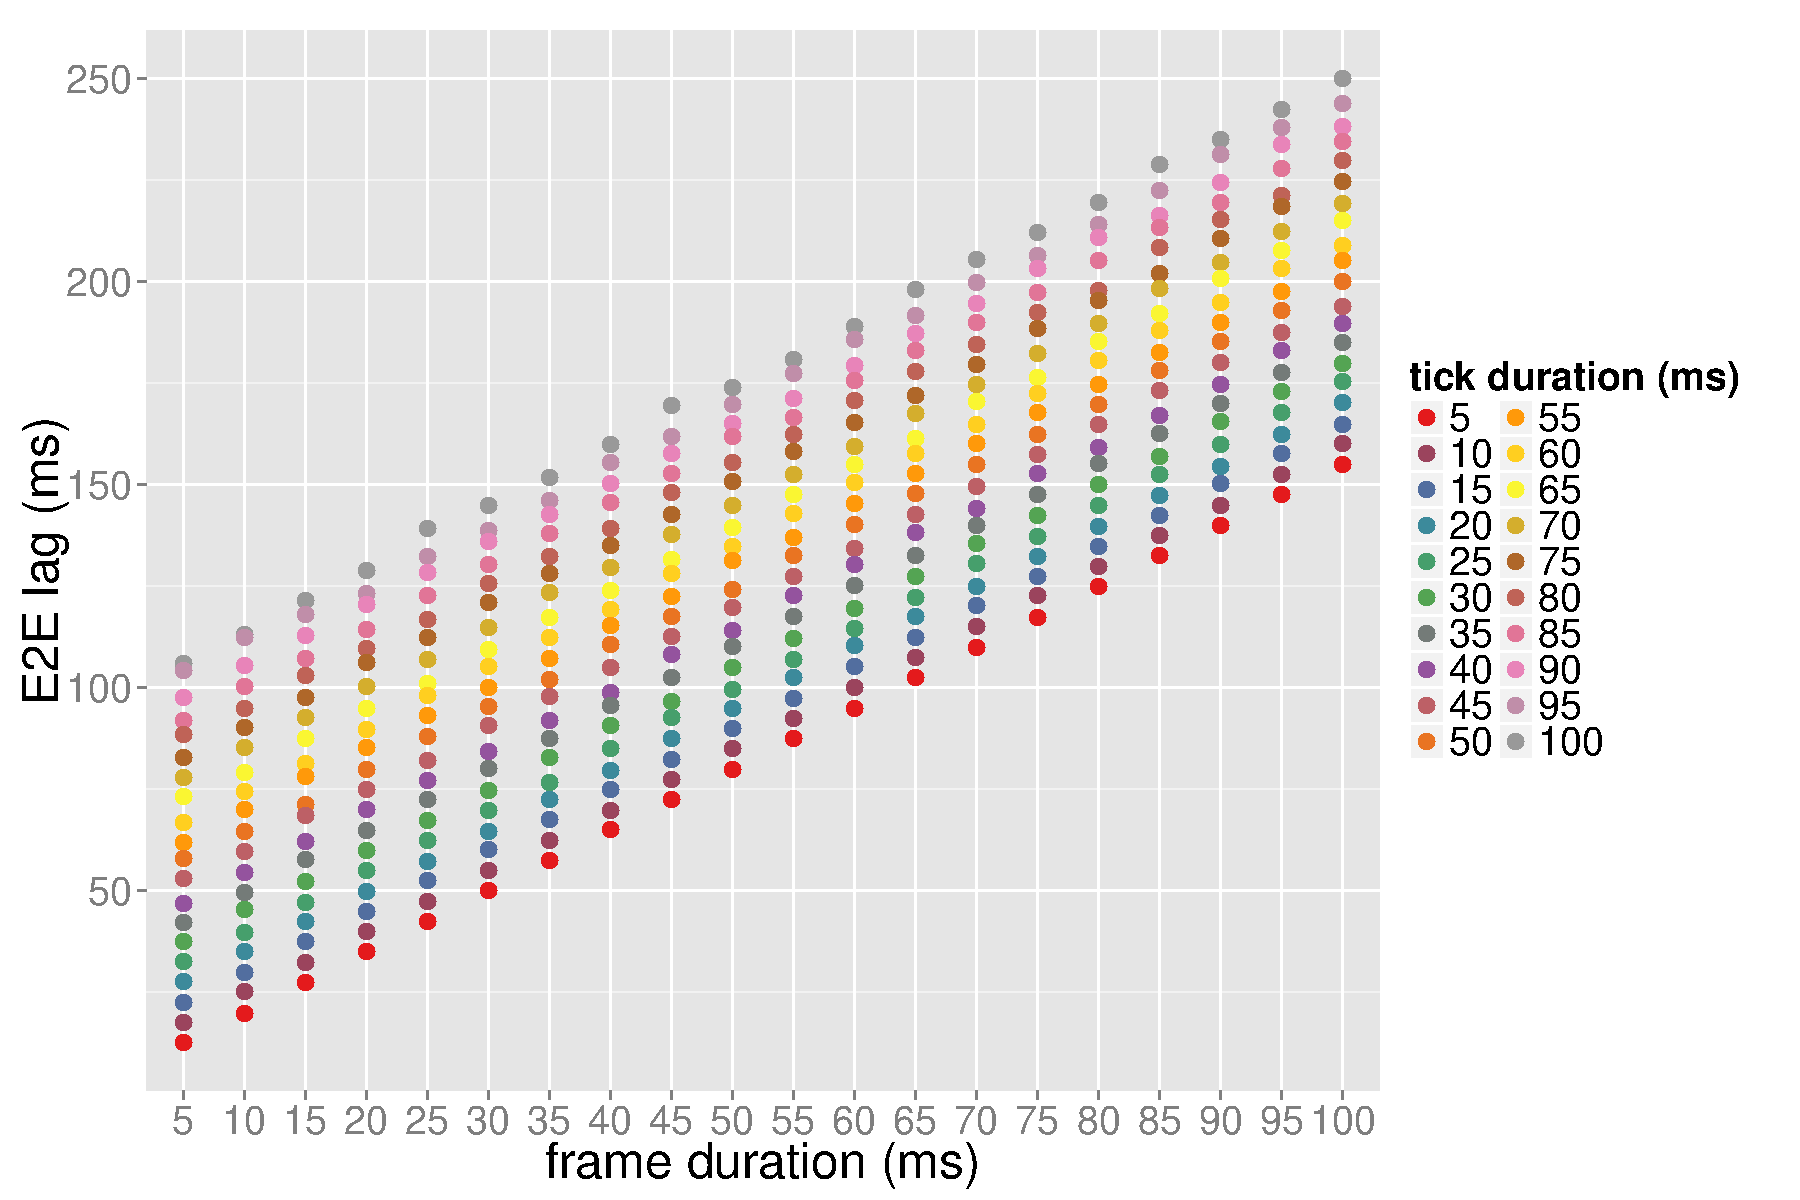
\includegraphics[width=1.0\columnwidth]{../simulation/visualization/nwless-onlinegame-1000rounds.pdf}
	\caption{Median end-to-end lag under various frame and tick durations for a locally-running game. Lower lag values are achieved at lower frame and tick durations.}
\label{fig:nwless-scatter}
\end{figure}

Figure~\ref{fig:nwless-scatter} plots the relationship between the frame duration (i.e., the inverse of the framerate), the tick duration, and the resulting median end-to-end lag.
% NOTA BENE: Every status update that the server sends must wait for another 
% frame time until we consider it rendered.
%
% The scatter plot of raw e2e lag values for one (FR, TR) configuration thus 
% spans
% * separate "boxes" for each CR/FR/TR offset config
% * inside of which the input events U scatter
% * Boxes are, when all other rates/processes are in optimal sync,
%   - bound from below by the frame-time f^-1 as the minimum
%   - bound from above by f^-1 + c^-1, because c "groups together" input events
% * alternatively, when maximally *out of* sync, 
%   - the boundaries shift upwards by another f^-1 + g^-1, resulting in 
%     a total just short of c^-1 + g^-1 + 2*f^-1:
%     Input event waits almost-full command cycle, which then waits 
%     almost-full tick, which then waits almost-full frame; plus one frame 
%     per the "nota bene" above.
% * a "cloud of boxes" (per the above description) whose minima are uniformly 
%   distributed (from visual inspection).
%
% The distributions of values for different (FR, TR) configs differ in 
% their characteristics pretty starkly:
% * for low framerates and high tickrates, we get an approximately 
%   uniform lag distribution. Seems that the FR which is "further down the 
%   tandem queue" dominates the lag, so its uniformly distributed phase 
%   offset governs the lag distribution.
% * for high framerates and low tickrates, it approaches a truncated 
%   normal distribution.
The values can be estimated as follows. Every user input 
event traverses three queues with fixed-rate outputs ($c=g$, g, and $f$), 
and every game state update waits for the next full frame until it gets 
displayed. In the ideal case, an input event occurs just before the command 
message is sent off, the server tick follows as soon as the message is 
received, and the update reaches the client just before a frame is output. 
Then the end-to-end lag is slightly above the frame time that must elapse 
before the update can be rendered to screen, $T_{min}>f^{-1}$.

In case the events are unfavorably offset against one 
another, an input event has to wait almost a full command-message cycle 
until it is sent on; it reaches the server just after a tick has 
occurred, so it waits almost a full server tick; finally, it will wait 
for almost two frame times until it is displayed. Combining with the 
previous result bounds the lag as follows, 
$f^{-1} < T < c^{-1}+g^{-1}+2f^{-1}$. The mid-interval point between 
these two limits is $T_{mid}=\frac{3}{2} f^{-1} + g^{-1}|_{c=g}$ which 
coincides roughly with the medians of the stochastic simulation.


Looking at a typical \SI{60}{\hertz} video game with an equal tickrate (i.e. a frame duration of $\approx \SI{16.6}{\milli\second}$) the median lag is in the range of \SIrange{45}{50}{\milli\second}. So even under quasi-optimal circumstances, there is already a considerable amount of end-to-end lag (even without factoring in the delay of the screen and input devices) that can only increase with the presence of network delay. Therefore, video games (and quality assessments thereof) should try to achieve the highest framerate possible to minimize this influence.

%%%%%%%%%%%%%%%%%%%%%%%%%%%%%%%%%%%%%%%%%%%%%%%%%%%%%%%%%%%%%%%%%%%%%%%%%%%%%%%%
\subsection{Online Gaming}

Next up is the full scenario of an online video game, now with 
network lag $D$ and server processing time $P$ included. For 
this exemplary scenario, the one-way delay $D$ was assumed to 
follow a left-truncated normal distribution, 
with $\mu_D = \SI{20}{\milli\second}$ and $\sigma_D = \SI{5}{\milli\second}$, 
producing non-negative network delays. Typical competitive online 
games today are expected to operate in such ranges. An 
\acrshort{RTT} of \SI{100}{\milli\second} is often considered to 
be the upper limit for a good playing experience.
$P$ is similarly left-truncated. In addition to the components in 
the previous scenario, the lag now also contains contributions by 
the network round-trip and processing delay, $2D + P$.

\begin{figure}[!t]
	% TODO: adjust the bounding box of the 3dbar plot, instead of playing with fire (aka \vspace)
	\centering
	\vspace{-6mm}
	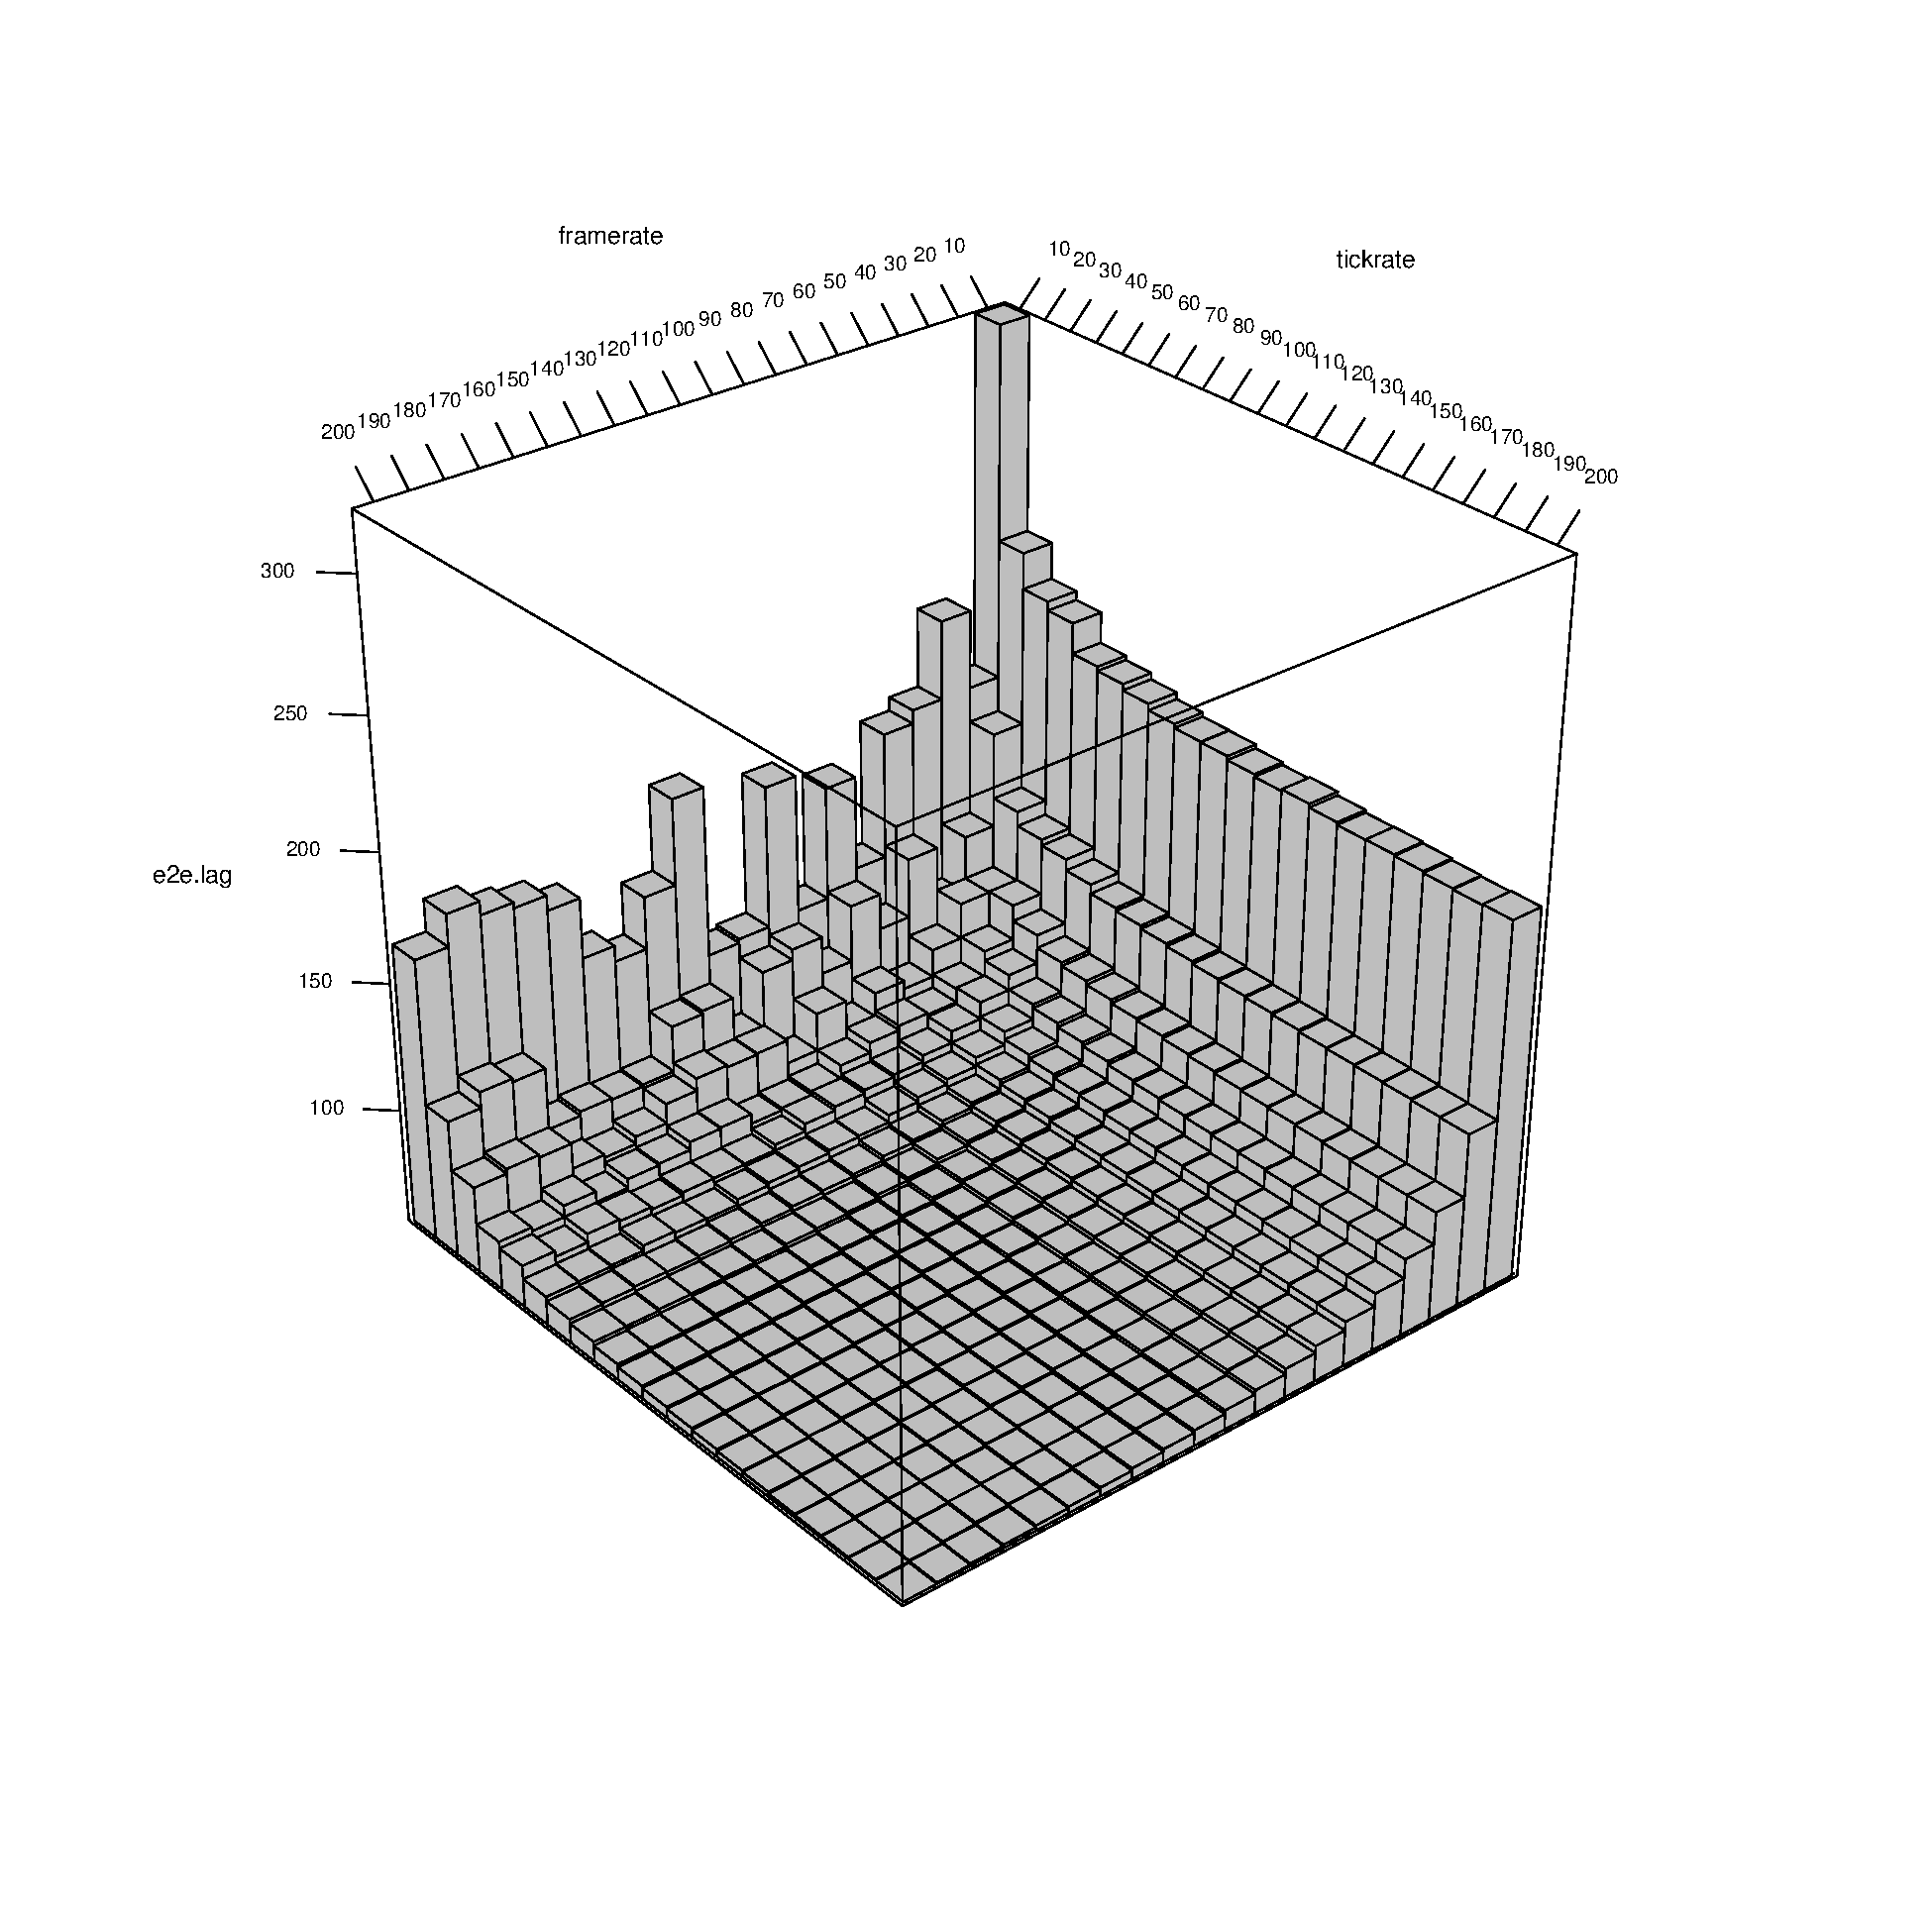
\includegraphics[width=1.0\columnwidth]{../simulation/visualization/e2e-lag-3dbars.pdf}
	\vspace{-15mm}
	\caption{Influence of client framerate and server tickrate on the median end-to-end lag in the online game scenario. For high rates $f$, $g$, the lag approaches $2\mu_D+\mu_P=\SI{43}{\milli\second}$.}
	% TODO: \hoss{Kann man hier einen stacked bar plot bauen, bei dem man den Networking Anteil sieht? Das wuerde die Aussage gut unterstuetzen.}
	% TODO: nicht rechtzeitig für submission deadline, aber für eine nächste version
\label{fig:3dbars-framerate-tickrate-lag}
\end{figure}

Figure~\ref{fig:3dbars-framerate-tickrate-lag} shows a 3D bar plot 
of the influence of both the framerate and the tickrate on this 
scenario. The axes mark typical values for $f$ and $g$. Two things 
can be noted here. First, the framerate has a larger influence on 
the lag than the tickrate. Second, for low framerates and tickrates, 
the impact of network delay on the end-to-end lag is almost 
completely masked. Only if both rates 
are high enough, the network delay will play a more significant role.
This masking effect has large implications for video games and their evaluation. Many evaluations examine the influence of the network delay only, without considering other contributions to end-to-end lag. Our results indicate that this might not be the best course of action. The effect likely shifts to lower values of the frame- and tickrates when a higher network delay is examined.

Another interesting result (not plotted here) is the much larger 
variance of lag in the framerate dimension when compared to the 
tickrate. This requires video game studies % experiments that examine the influence of the framerate need 
to have a very high repetition rate to %keep the variance low and 
provide meaningful results.


%%%%%%%%%%%%%%%%%%%%%%%%%%%%%%%%%%%%%%%%%%%%%%%%%%%%%%%%%%%%%%%%%%%%%%%%%%%%%%%%
\subsection{Cloud Gaming}

Finally, we construct a Cloud Gaming scenario. The tickrate has been 
removed;  instead, a constant encode ($e$) and decode ($d$) delay is 
in place at the game streaming server and client respectively. 
The frames are now rendered by the server, so they need to be 
transported back to the client first. 
Instead of assuming a specific network throughput and frame size, 
we simply add one frame time to account for the transmission 
of the encoded screen contents.
%Without knowing the connection's throughput and absolute values for the frame sizes, the simulation simply applies an upper limit for the transmission duration, namely once again the frame's duration, or the inverse of the framerate. 
For the network delay $D$, the same values as for the online game are used.
$c$ is set to $\SI{200}{\hertz}$.

\begin{figure}[!t]
	\centering
	%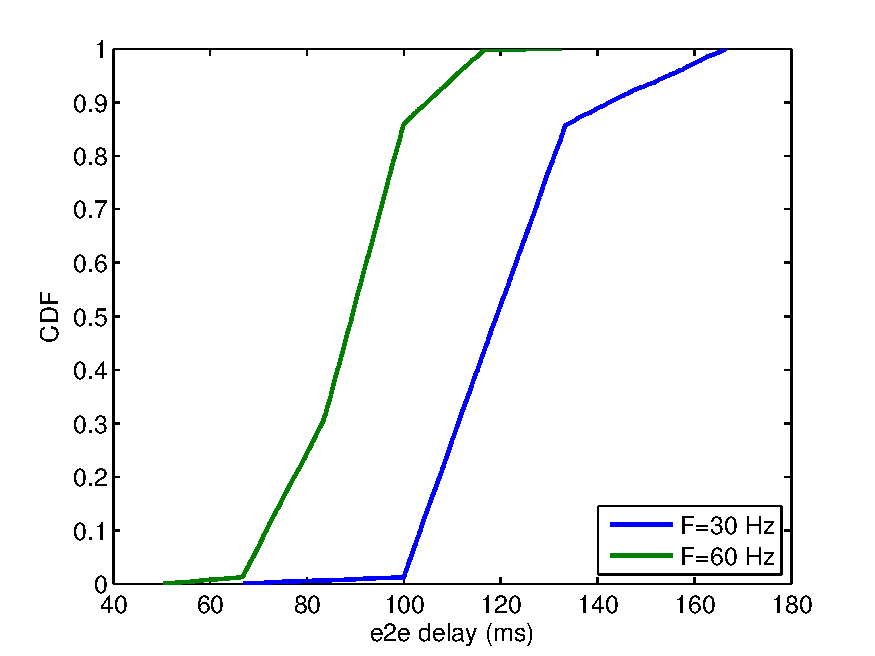
\includegraphics[width=1.0\columnwidth]{images/e2e-delay-sim.pdf}
	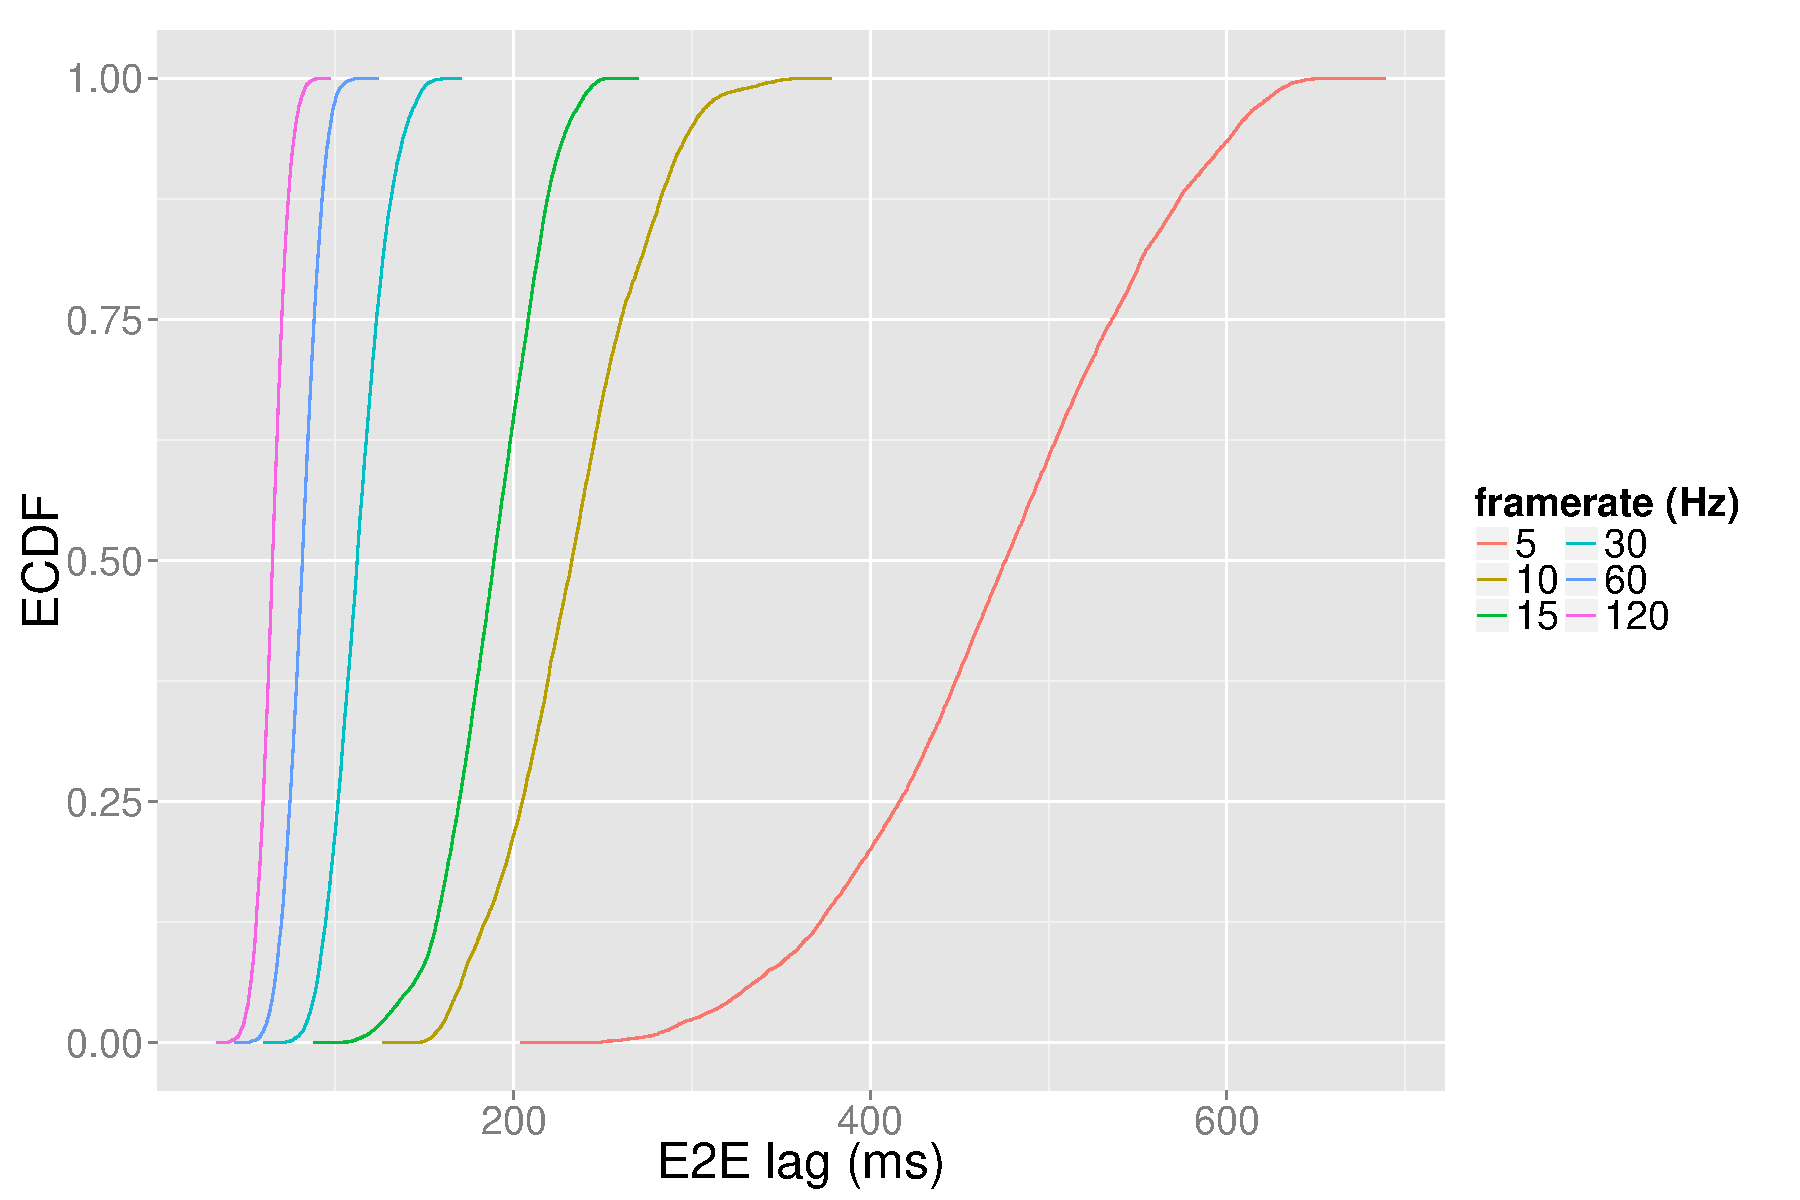
\includegraphics[width=1.0\columnwidth]{../simulation/visualization/cloudgaming-lag-cdf.pdf}
	\caption{\acrshort{ECDF} of the influence of the rendering and streaming framerate on the end-to-end lag in the cloud scenario. Vertical intercept denotes the average base delay of $\SI{68}{\milli\second}=\inv{c}+2D+P+e+d$.}
	%\hoss{On average, a network delay of $\unit[2\cdot20=40]{ms}$ (correct???) exists. A constant encoding time (\unit[15]{ms}) and decoding time (\unit[5]{ms}) is assumed. Thus, the major part of the e2e lag is caused by the framerate setting. Kann man hier noch eine Linie reinzeichnen, die die Summe 5+15+40=60 ms zeigt?}}
	%
	% Albert: Uh, oh, the cloud simulation seems to have reused a stray 
	%         200 Hz setting for $c$ from a previous online game sim.
	%         I'm documenting that this value has been used.
	%
\label{fig:cloud-e2e-delay-sim}
\end{figure}

Figure~\ref{fig:cloud-e2e-delay-sim} shows the results of this scenario 
as an \gls{ECDF} of the end-to-end lag for several framerates. As before, 
the framerate impacts the end-to-end lag more severely than the network delay.
%the large influence of the framerate when compared to the network delay is evident. 
This result is of particular importance considering how past studies 
have relied on similarly low framerates as $5-\SI{15}{\hertz}$ when 
assessing the network influence on cloud gaming.
Similarly, these results can provide guidelines for implementors of 
cloud gaming to factor in the framerate in their calculations accordingly.


%%%%%%%%%%%%%%%%%%%%%%%%%%%%%%%%%%%%%%%%%%%%%%%%%%%%%%%%%%%%%%%%%%%%%%%%%%%%%%%%
\subsection{Discussion}

The three scenarios presented here serve to provide initial insights into the complex interactions of the end-to-end lag. Although the underlying abstract model adopts some simplifications and some properties are not factored in yet, the results are still very revealing.
Using the model and simulator as baseline, one can get a good estimation of the expected video game \gls{QoS} values. Alternatively, it can help in choosing representative games for select scenarios.

% Ultimately, to capture any and all latency sources in gaming you would need to rely on external recording gear.
% With modified input: zero latency and visible input detection (e.g. solder some LEDs to the buttons)

% Also Arduino with photodiode method described in \cite{beyermethod}
% Both this and camera method also work for closed game consoles


%%%%%%%%%%%%%%%%%%%%%%%%%%%%%%%%%%%%%%%%%%%%%%%%%%%%%%%%%%%%%%%%%%%%%%%%%%%%%%%%
%\subsection{Evaluated Metrics}

%%%%
%\subsubsection{Frame Rates and Frame Times (i.e. frame IAT)}
%i.e. frame IAT
%Reasoning for frame IAT and the negligence of past investigations
%%%%
%\subsubsection{Total and additional end-to-end latency}
%physical controller input to in-game reaction
%different in-game actions have already difference in latency, therefore need to test various actions for a complete picture
%Also discuss RTT as Hz (1/RTT) as measure for interactivity


%%%%%%%%%%%%%%%%%%%%%%%%%%%%%%%%%%%%%%%%%%%%%%%%%%%%%%%%%%%%%%%%%%%%%%%%%%%%%%%%
%\subsection{Reasonable Configuration/Setting Ranges to Test}

% Resolution: Minimum 720p, 1080p recommended, even higher is better (1440p or 2160p)
% Frame rate: 60 fps very much recommended, 30 absolute minimum,  120 or 144 can also be feasible
% Configure games to run at high or at least medium settings
% For console games: use the games intended settings for the console, never downscale the game or reduce the frame rate for streaming
% Assume no network latency higher than 200ms, preferably less than 100ms
% Assume typical access link conditions, i.e. no less than 10-16Mb/s



%Works only for general purpose computing devices with full access.
%Easiest method, but might not capture full end-to-end latency.
%FRAPS, OBS, DirectX Hooking, MSI Afterburner
%FCAT as hybrid solution with external capture card and computer


% \url{http://www.red.com/learn/red-101/high-frame-rate-video}


% articles:
% why frametimes
%     \url{https://techreport.com/review/21516/inside-the-second-a-new-look-at-game-benchmarking}

% Inside the second with Nvidia's frame capture tools
%     \url{https://techreport.com/review/24553/inside-the-second-with-nvidia-frame-capture-tools}

 % As the second turns: the web digests our game testing methods
 %    \url{https://techreport.com/blog/24133/as-the-second-turns-the-web-digests-our-game-testing-methods}

% GPU Reviews: Why Frame Time Analysis is important
%     \url{http://www.vortez.net/articles_pages/frame_time_analysis.html}

% Durante's Witcher 3 analysis: the alchemy of smoothness
%     \url{http://www.pcgamer.com//durantes-witcher-3-analysis-the-alchemy-of-smoothness/}


% Analysing Stutter – Mining More from Percentiles
%     \url{https://developer.nvidia.com/content/analysing-stutter-%E2%80%93-mining-more-percentiles-0}

% fraps vs fcat method
%     \url{http://www.extremetech.com/gaming/154089-after-almost-20-years-gpu-benchmarking-is-moving-past-frames-per-second}

% FRAPS + FRAFS
% \url{http://www.fraps.com/}
% \url{http://sourceforge.net/projects/frafsbenchview/}
% \url{http://www.5group.com/wordpress/2012/07/14/gpu-mist-pre-release-1-0-rc1/}

% issue: Fraps measures the flip queue input rather then the actual render output frames which is fine when measuring FPS but is rather poor if you want to measures actual frame times and analyze microstutter.


% NVIDIA FCAT
% \url{http://www.geforce.com/hardware/technology/fcat}
% \url{http://www.overclockers.com/nvidias-fcat-gpu-testing-pursuing/}


% Valve for Linux GL Games
% \url{https://github.com/ValveSoftware/voglperf}

% Info über MSI Afterburner overlay? oder GF experience? GPU-Z? Rivatuner Statistics Server?
% \url{http://www.overclock.net/a/how-to-use-rivatuner-afterburner-on-screen-display-and-more}



% \url{https://en.wikipedia.org/wiki/Game_classification}
% \url{https://en.wikipedia.org/wiki/Video_game_genre}
% \url{https://en.wikipedia.org/wiki/List_of_video_game_genres}

